\section{Results}
The graph below are the result of two neural network, one with TanH layer and one with ReLu layer, with the following parameters :
$2$ input, $2$ output and $3$ hidden layer of $25$ neuron each, $200$ epochs, batch size of $1$ and a learning rate of $0.02$. The training set is $1000$ random two dimensional points between $0$ and $1$ classified with a $1$ if the point is in a circle center in $[0.5,0.5]$ and radius equal to $1/\sqrt{2\pi}$ and $0$ when the point are outside. A seed is use for the random generation for the parameters to have always value to help to debug and compare the result. The complete code is in the appendix~\ref{app::code}.
\begin{figure}[H]
	\begin{subfigure}[h]{0.4\textwidth}
		\begin{center}
			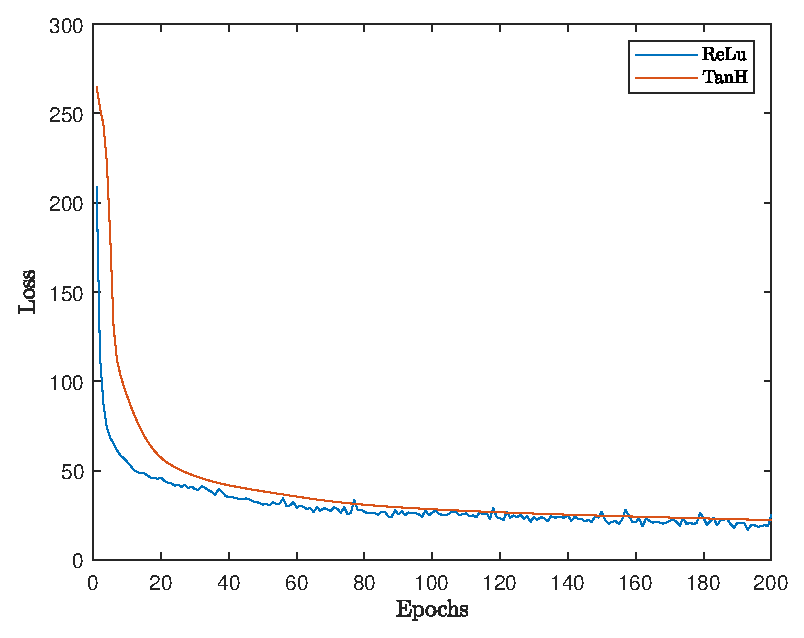
\includegraphics[width=\textwidth]{loss200}
			\caption{Loss}
		\end{center}
	\end{subfigure}
	\begin{subfigure}[h]{0.4\textwidth}
		\begin{center}
			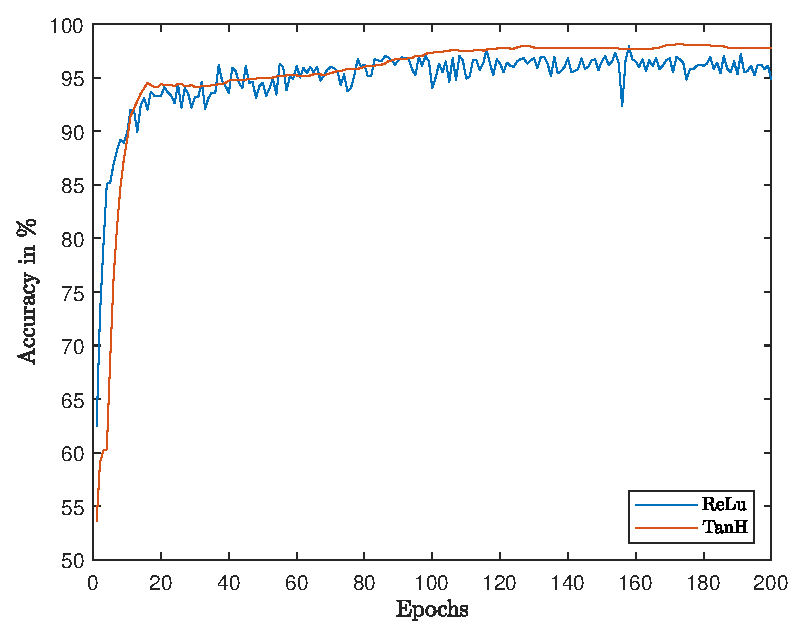
\includegraphics[width=\textwidth]{accuracy200}
			\caption{Accuracy}
		\end{center}
	\end{subfigure}
	\begin{subfigure}[h]{0.4\textwidth}
		\begin{center}
			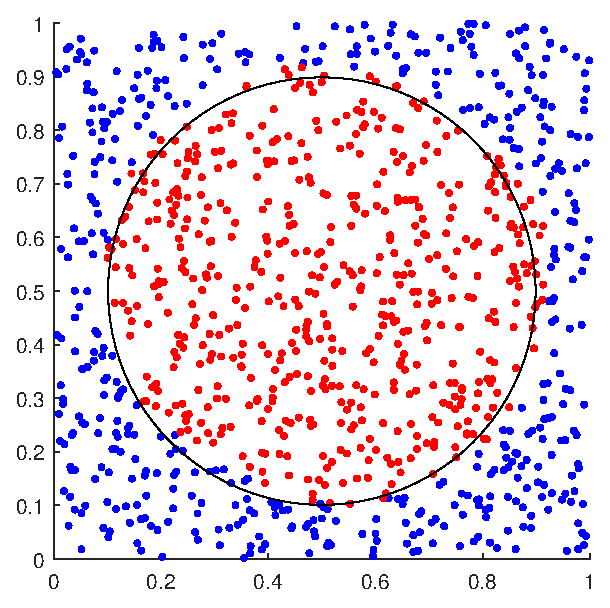
\includegraphics[width=\textwidth]{relu_out}
			\caption{Test set classified with ReLu}
		\end{center}
	\end{subfigure}
	\begin{subfigure}[h]{0.4\textwidth}
		\begin{center}
			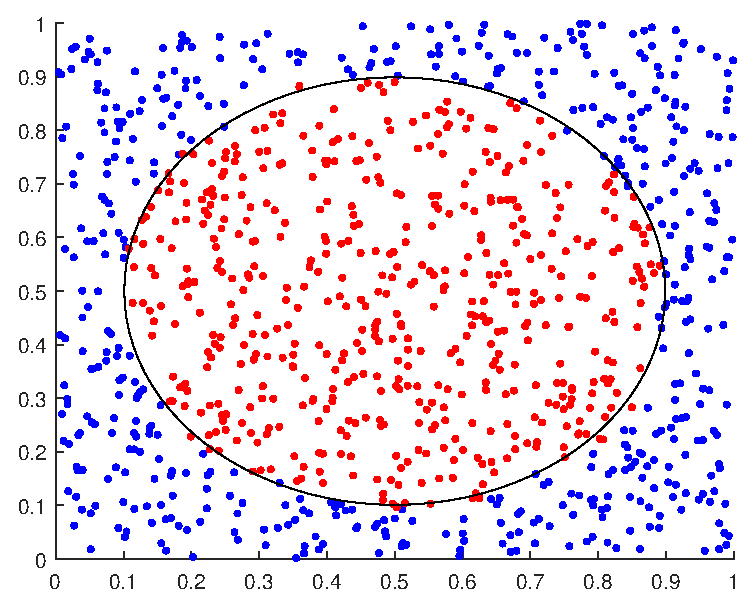
\includegraphics[width=\textwidth]{tanh_out}
			\caption{Test set classified with TanH}
		\end{center}
	\end{subfigure}
	\caption{Result of two neural network with ReLu and TanH layer with the following parameters : $2$ input, $2$ output and $3$ hidden layer of $25$ neuron each, $200$ epochs, batch size of $1$ and a learning rate of $0.02$}
	\label{img::result}
\end{figure}

The final error rate for the ReLu neural network with the test set is $5.8\%$, and $2.2\%$ with the TanH neural network.